\chapter{Ergebnisse}

Zum Abschluss dieser Arbeit wird eine kurze Erklärung von Ergebnissen zusammengefasst. Wie in der \autoref{fig:optocoupler} zu sehen ist, wird ein kontinuierlich-sinusförmiges Signal an den Pin $A$ und Pin $B$ des Optokopplers angeschlossen. Das vom Frequenzgenerator generierte Signal wird in der \autoref{fig:sinus} dargestellt. Die Diode $D1$ spielt hier eine wichtige Rolle, damit der Strom von $B$ nach $A$ fließen kann. Danach wird das Eingangssignal des Optokopplers zwischen den Pin $1$ und Pin $2$ am Oszilloskop gemessen, wie in der \autoref{fig:input} zu sehen ist. Anschließend wird das Eingangssignal mit Hilfe des Optokopplers am Ausgangspin als \textit{digitalisiertes Signal} entnommen, wie in der \autoref{fig:digital} dargestellt wird. \smallskip \smallskip

\begin{figure}[htbp]
	\centering
	\fbox{
		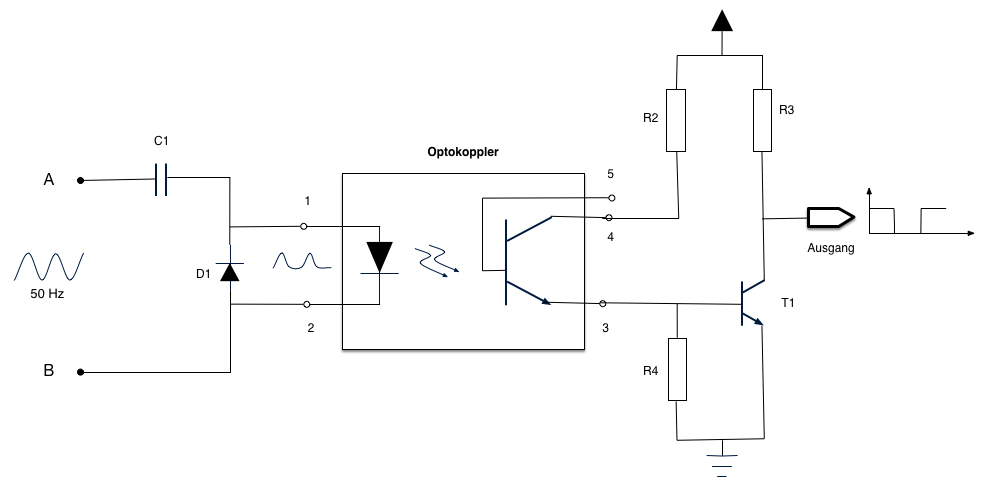
\includegraphics[width=300px,height=160px]{pictures/fazit/optocoupler.png}
	}
	\caption{Schaltplan des Optokopplers}\label{fig:optocoupler}
\end{figure} 

\begin{figure}[ht!]
     \begin{center}
        \subfigure[Sinusförmiges Signal vom Frequenzgenerator]{%
           \label{fig:sinus}
           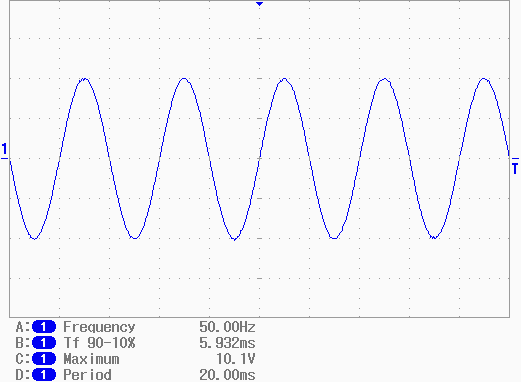
\includegraphics[width=0.45\textwidth]{pictures/fazit/sinus.png}
        }%\\ %  ------- End of the first row ----------------------%
        \subfigure[Eingangssignal des Optokopplers]{%
            \label{fig:input}
            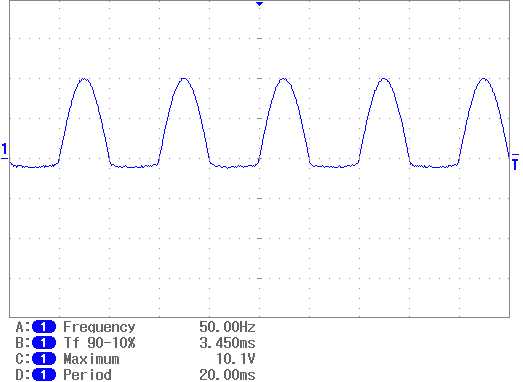
\includegraphics[width=0.45\textwidth]{pictures/fazit/input.png}
        }\\ %
        \subfigure[Digitalisiertes Ausgangssignal des Optokopplers]{%
            \label{fig:digital}
            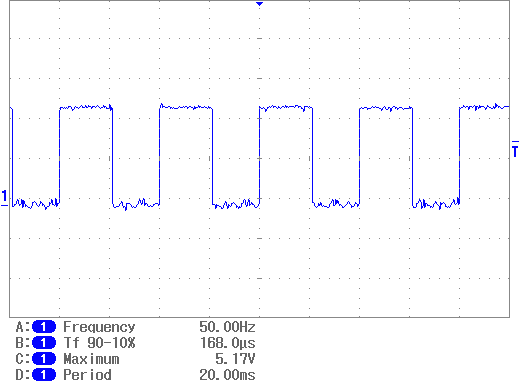
\includegraphics[width=0.45\textwidth]{pictures/fazit/digital.png}
        }%
%
    \end{center}
    \caption{Eingangs- und Ausgangssignale des Optokopplers}%
   \label{fig:signals}
\end{figure}

Am Schluss wird das digitalisierte Signal an den Eingangspin des ATMega16-Mikrocontrollers weitergeleitet. Wenn eine fallende Flanke am Pin des Mikrocontrollers eintrifft, wird der Timer-Interrupt ausgelöst, in dem der Timer-Wert in eine vordefinierte Variable gespeichert wird. Im nächsten Interrupt wird die Differenz zwischen zwei aufeinanderfolgenden fallenden Flanken gespeichert. In der Firmware wird ein Ringpuffer\footnote{ist ein Datenspeicher mit $N$ Datenelementen, wobei der Zeiger ringförmig auf die Datenelemente zeigt.} erstellt, indem die gemessenen Zeitdifferenzen sich befinden. Bei der Abfrage der Frequenz aus dem UNIX-Server werden alle Zeitdifferenzen aus dem Ringpuffer ausgelesen und der Mittelwert berechnet, wie in der folgenden Formel beschrieben wird:

\begin{align}
	Mittelwert = \frac{\sum_{i=1}^{N} Puffer[i]}{N}
\end{align}

wobei $N$ die Länge des Ringpuffers ist. Um die Mittelfrequenz zu berechnen, wird die Taktfrequenz des ATMega16-Mikrocontrollers verwendet, wie in der folgenden Formel beschrieben wird:

\begin{align}
	Mittelfrequenz = \frac{F\_CPU}{Mittelwert * Timer\_Vorteiler}
\end{align}

wobei $F\_CPU$ mit $16$ MHz bestimmt ist, und der $Timer\_Vorteiler$ als $256$ definiert wurde. \smallskip \smallskip 

Nach der Kompilierung der Firmware sieht die Ausgabe folgendemaßen aus:

\begin{minted}[linenos=false, frame=single, fontsize=\scriptsize]{text}
 --- --- --- Target  Information --- --- --- 
      AVR Model       : atmega16
      Board           : Frequenzmessung
      MCU Frequency   : 16000000 Hz
 --- --- --- --- --- --- --- --- --- --- --- 

Size after:
===========================
main.elf  :
section           size      addr
.text             5970         0
.data               12   8388704
.bss               211   8388716
.comment            17         0
.debug_aranges     456         0
.debug_info       9127         0
.debug_abbrev     2740         0
.debug_line       2493         0
.debug_frame      1600         0
.debug_str        1127         0
.debug_loc        5429         0
.debug_ranges       48         0
Total            29230

AVR Memory Usage
----------------
Device: atmega16

Program:    5982 bytes (36.5% Full)
(.text + .data + .bootloader)

Data:        223 bytes (21.8% Full)
(.data + .bss + .noinit)
\end{minted} 

Mit dem \code{ping}-Programm wird eine Abfrage aus dem UNIX-Server an den ENC28J60-Mikrochip gesendet, ob er im Netz verfügbar ist. Es wurde in dieser Arbeit kein DHCP-Protokoll erstellt. Aus diesem Grund muss die IP-Adresse des Mikrochips in der Firmware manual eingetragen werden. Die IP-Adresse ist in der \code{main}-Datei als ''192.168.0.3'' definiert. Wenn der Mikrochip eine richtige IP-Adresse im lokalen Netz besitzt, dann liefert der Mikrochip nach der \code{ping}-Abfrage folgende Antwort zurück: 

\begin{minted}[linenos=false, frame=single, fontsize=\scriptsize]{bash}
$ ping -c 5 192.168.0.3
PING 192.168.0.3 (192.168.0.3): 56 data bytes
64 bytes from 192.168.0.3: icmp_seq=0 ttl=64 time=0.788 ms
64 bytes from 192.168.0.3: icmp_seq=1 ttl=64 time=0.438 ms
64 bytes from 192.168.0.3: icmp_seq=2 ttl=64 time=0.464 ms
64 bytes from 192.168.0.3: icmp_seq=3 ttl=64 time=0.529 ms
64 bytes from 192.168.0.3: icmp_seq=4 ttl=64 time=0.587 ms

--- 192.168.0.3 ping statistics ---
5 packets transmitted, 5 packets received, 0.0% packet loss
round-trip min/avg/max/stddev = 0.438/0.561/0.788/0.125 ms
\end{minted}

Wenn aber der Mikrochip keine gültige lokale IP-Adresse definiert hat, liefert der Mikrochip nach der \code{ping}-Abfrage folgende \textit{Zeitüberschreitungsmeldung}:  \smallskip \smallskip

\begin{minted}[linenos=false, frame=single, fontsize=\scriptsize]{bash}
$ ping -c 5 192.168.0.3
PING 192.168.0.3 (192.168.0.3): 56 data bytes
Request timeout for icmp_seq 0
Request timeout for icmp_seq 1
Request timeout for icmp_seq 2
Request timeout for icmp_seq 3
Request timeout for icmp_seq 4

--- 192.168.0.3 ping statistics ---
5 packets transmitted, 0 packets received, 100.0% packet loss
\end{minted}

Mit dem UNIX-Dämon wird eine Abfrage über das UDP-Protokoll gesendet, um die Mittelfrequenz aus dem ENC28J60-Mikrochip zu erhalten. Der Dämon hat zwei Argumente, IP-Adresse und die Portnummer. Die Argumentbehandlung wird im folgenden Code-Feld beschrieben:  \smallskip \smallskip

\begin{minted}[linenos=false, frame=single, fontsize=\scriptsize]{bash}
$ ./daemon 
Usage: 
	./daemon -h <hostname> -p <port>
	Example: ./daemon -h FreeBSD.local -p 32000
\end{minted}

Wie schon beschrieben wurde, wurde in der Firmware die IP-Adresse ''192.168.0.3'' und die Portnummer ''1200'' definiert. Aus diesem Grund wird der UNIX-Dämon wie in dem folgenden Code-Feld verwendet:

\begin{minted}[linenos=false, frame=single, fontsize=\scriptsize]{bash}
$ ./daemon -h 192.168.0.3 -p 1200
hostname: 192.168.0.3
port number: 1200
sending: start
waiting for packet ...
received packet from 192.168.0.3: 50.153 Hz
\end{minted}

Wie in der letzten Zeile des obigen Code-Felds zu sehen ist, hat der Mikrochip nach der Abfrage die Mittelfrequenz als \textit{50.153 Hz} gesendet bzw. beantwortet.


